\chapter{Experimentos}

\section{Análise Exploratória}

\subsection{Distribuição das classes}

Antes de mais nada, analisaremos a composição do nosso conjunto de dados e como se dá
a distribuição de classes. Na figura \ref{fig:classes} temos um histograma das classes associadas
a cada tuíte.

\begin{table}[H]\label{tab:distribution}
	\begin{center}
		\begin{tabular}{| l | l |}
			\hline
			Positivo & 115 \\ 
			Negativo & 1248 \\ 
			Neutro & 1223 \\ 
			\hline
		\end{tabular}
	\end{center}
	\caption*{Quantidade de tuítes pertencentes a cada classe}
\end{table}

\begin{center}
	\begin{figure}[H]\label{fig:classes}
		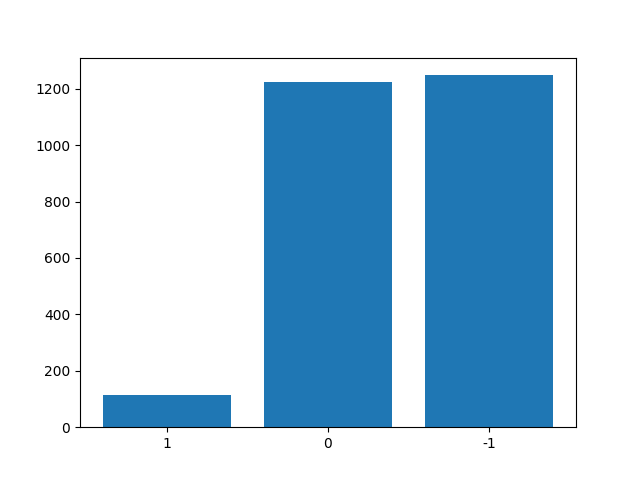
\includegraphics[scale=0.8]{fig_classes}
		\caption{Histograma da frequência de tuítes}
	\end{figure}
\end{center}

Como podemos observar a partir da figura \ref{fig:classes} e tabela \ref{tab:distribution}, temos
que enquanto as classes negativa e neutra possuem distribuição próxima (48,26\% e 47,29\% 
respectivamente) a classe positiva corresponde a apenas 4,45\% de todos os tuítes. Mais a frente
veremos que esse desbalanceamento entre as classes irá acarretar em um desempenho ruim por parte
dos algoritmos de classificação, sejam os desenvolvidos para este trabalho quanto os da biblioteca
\texttt{scipy}.

\subsection{Características dos tuítes de cada classe}

A fim de entender como os classificadores realizariam o treinamento, analisou-se o conjunto de
dados a procura de padrões de características para cada classe.

Para os tuítes avaliados como neutro, notou-se o padrão que são tuítes derivados de portais de 
notícias ou são indagações, porém sem nenhuma crítica feita nelas.
A tabela abaixo mostra como exemplo alguns tuítes avaliados como neutro.

\begin{center}
	\begin{tabular}{| l | p{0.8\linewidth} |}
		\hline
		usuário & tuíte \\
		\hline
		Tica_Fernandes & Cidades têm protestos contra reforma da Previdência e terceirização http://g1.globo.com/politica/noticia/cidades-tem-protestos-contra-reforma-da-previdencia-e-terceirizacao.ghtml \\
		\hline
		andrcolett & Transposição do rio São Francisco, reforma do ensino médio/ da previdência , operação carne fraca, terceirização ... Enem vai bombar esse ano \\
		\hline
		VictoorAugustoo & Via @estadao : Manifestantes protestam em capitais do País contra reforma da Previdência e terceirização - http:/ln.is/estadao.com.brb29w1 \\
		\hline
		EdmilsonPequeno & O meu deputado @luizcoutopt votou contra a terceirização e é contra a reforma da previdência \\
		\hline
	\end{tabular}
\end{center}

Já para os tuítes negativos, nota-se a presença de palavrões e xingamentos 
junto de algumas \textit{hashtags} de cunho negativo como por exemplo \#ForaTemer,
além disso é comum a presença de tuítes onde as pessoas são convocadas para manifestações.
Outros termos comuns são escravidão e retrocesso, referindo-se diretamente às reformas da previdência e terceirização.

\begin{center}
	\begin{tabular}{| l | p{0.8\linewidth} |}
		\hline
		usuário & tuíte \\
		\hline
		MgracaGalvao & Dória é o maior Fake de todos os tempos. Se f... Palhaço \\
		\hline
		adamastaquio & Acorda POVO trabalhador. Previdencia + Terceirização + Reforma da CLT é P*** NO RABO DO POVO! \#ReformaTrabalhistaNÃO \\
		\hline
		TheMairaBastos & Reforma da previdência , desmonte da CLT, terceirização ,congelamento de gastos com a saúde e educação \#ForaTemerLadrao \#TemerGolpista \\
		\hline
		neyeverest & O PT esteve no poder por 14 anos o bandido do Lula e a burra da Dilma e o país está um caos pela instituição a roubalheira deles também !! \\
		\hline
		carinasotero & GREVE GERAL DIA 28/04 CONTRA RETROCESSOS DE TEMER • Reforma da Previdência • Reforma Trabalhista • Terceirização irrestrita \\
		\hline
	\end{tabular}
\end{center}

Assim como para os tuítes classificados como negativo, os tuítes positivos também eram 
caracterizados pela presença de \textit{hashtags}. Sejam elas declarando apoio a um candidato
(como \#Aecio2018 ou \#Lula2018) ou simplesmente manifestando alguma opinião positiva. 

\begin{center}
	\begin{tabular}{| l | p{0.8\linewidth} |}
		\hline
		usuário & tuíte \\
		\hline
		Verinha_Lu & É Aécio pelo Brasil !!! \#AécioPresidenteDoBrasil2018 \#EstamosComAécio \#DeusÉmaior e \#VitóriaVem \#FÉ \#SouAécio \\
		\hline
		Haddad_Femando & O salário mínimo aumentou 71\% durante os governos Lula e Dilma \#BrasilQueOPovoQuer \\
		\hline
		rovisacro & A favor da terceirização e tmb da reforma da previdência ! Mas óbvio, de forma justa e igualitária para todos, principalmente na previdência \\
		\hline	
	\end{tabular}
\end{center}

\section{Descrição dos experimentos}

Para cada classificador, realizou-se experimentos tomando como base não só

\section{Métricas avaliadas}

Para a realização dos experimentos, levou-se em consideração três métricas
para avaliar a eficiência dos classificadores.